%Gliederung:
%
%Abstract
%Einleitung <--- Martin
%       Geschichte
%        Wozu, Verbreitungsgrad
%        Anwendungsgebiete
%Funktionsweise: Aufbau von PPP <--- Michael Sch.
%        Header, Payload
%        (Verschiedene Arten von PPP)
%        Unterprotokolle
%Ablauf von PPP-Verbindungen <--- Michael St.
%        Schwerpunkt PPPoE
%Schlussfolgerung
%
% Zu beachten:
% - 6 pages including pictures and references
% - Wikipedia is not an allowed reference
% - And do not use pictures or examples that you can find in the exercises or the lecture.
\documentclass[journal]{IEEEtran}
\usepackage[utf8x]{inputenc}
\hyphenation{op-tical net-works semi-conduc-tor} 
\usepackage[pdftex]{graphicx}
\begin{document} 
\title{Das Grundprinzip von PPP - \\wie es funktioniert, pros und cons} 
\author{\IEEEauthorblockN{Martin Hellwig, Michael Schulze, Michael Stahn}
\IEEEauthorblockA{\\Kommunikationsnetze 1\\ Technische Universit\"at Darmstadt\\} }
\maketitle 
\begin{abstract} 
Diese Arbeit behandelt das Thema Point-to-Point Protocol (PPP). Dieses Protokoll wurde als Ersatz f\"ur fr\"uhere Einwahlprotokolle entwickelt. Heutzutage findet es seine Hauptanwendung beim Einw\"ahlen via DSL. Neben der technischen Umsetzung und Spezifikation wird in dieser Arbeit auch ein m\"oglicher Verbindugsaufbau via PPP gezeigt.
\end{abstract} 
\begin{IEEEkeywords} 
PPP, PPPoE, PPPoA, Point-to-Point. 
\end{IEEEkeywords}
\section{Einleitung} 
\IEEEPARstart{D}{as} Point-to-Point Protocol wurde urspr\"unglich im Jahr 1994 von W. Simpson entwickelt. Im OSI-Modell ist es zusammen mit anderen Protokollen in der DataLink-Schicht daf\"ur zust\"andig eine direkte Verbindung zwischen zwei Clients \"uber ein leitungsvermittelndes Netz herzustellen. F\"ur diesen Zweck werden auch M\"oglichkeiten der Authentifizierung spezifiziert \cite{RFC1661}. Ebenfalls besteht die M\"oglichkeit die Daten zu verschl\"usseln oder zu komprimieren. Die Protokolle der OSI-Netzwerk-Schicht k\"onnen dann die bestehende PPP-Verbindung zur \"Ubermittlung von Daten nutzen. Eine PPP-Verbindung (beispielsweise zwischen ISPs, Routern, Hosts oder Netzwerkbr\"ucken) ist eine Full-Duplex Verbindung und versucht die zu \"ubermittelnden Pakete in der richtigen Reihenfolge zu \"ubertragen.\\
Die Notwendigkeit dieses Protokolls war zu dieser Zeit sehr hoch, da \"altere Standards, wie beispielsweise SLIP, nicht mehr zeitgem\"a\ss{} waren. Ebenfalls wurde der Telefon-Standard "Link Access Protocol, Balanced", welcher in der X.25-Protokollfamilie benutzt wurde, durch PPP ersetzt.  Speziell f\"ur die Internetverbindung f\"ur Heimanwender wurde f\"ur den alten ISDN-Standard ein Ersatz erschaffen. Eine Eigenschaft des Point-to-Point Protokolls ist es, f\"ur andere Protokolle der Netzwerk-Schicht leicht zu bedienen und zu nutzen zu sein. Mit den beiden Unter-Protokollen PPPoE (Point-to-Point over Ethernet)\cite{RFC2516} und PPPoA (Point-to-Point over ATM)\cite{RFC2364} kann man sich nun mithilfe eines Routers direkt mit dem Provider verbinden, was h\"ohere Datenraten zul\"asst. Dabei bleibt aber weiterhin der Vorteil (welcher zum Beispiel bei ISDN vorhanden ist), dass man zeitgebundene Tarife f\"ur die Endkunden anbieten und abrechnen kann. Bei heutigen DSL-Anschl\"ussen besitzt man zwar eine dauerhafte physikalische Verbindung zum Provider, doch erst mit dem Aufbau der PPP-Verbindung ist man auch virtuell mit dem Provider verbunden und kann somit das Internet nutzen. Nicht nur f\"ur heimische Internet-Anschl\"usse wird PPP genutzt, sondern in allen Netzwerkverbindungen, in welchen man sich erst einw\"ahlen muss. Dazu geh\"ort auch das Mobilfunktnetz oder auch die Einwahl \"uber eine ISDN-Verbindung.\\
In folgendem Bild (siehe Bild \ref{fig:PPP-Visualisierung}) wird gezeigt f\"ur welchen Zweck das PPP-Protokoll bei DSL-Zug\"angen genutzt wird. Dabei stellt der heimische Router eine feste virtuelle Verbindung zu der Gegenstelle des Providers her, welche (aktuell in Deutschland so geregelt) im Normalfall alle 24 Stunden neu aufgebaut wird, da dann die Verbindung seitens des Anbieters automatisch getrennt wird. \\
\begin{figure}[h!]
 \centering
  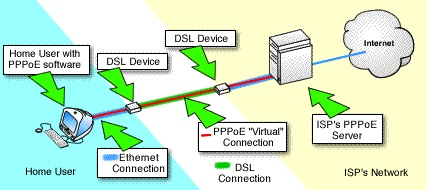
\includegraphics[width=0.5\textwidth]{img/PPP-Visualisierung}
 \caption{Darstellung einer PPP-Verbindung zwischen Heimanwender und ISP (Entnommen aus \cite{PPP-Bild})}
 \label{fig:PPP-Visualisierung}
\end{figure}
Neben DSL-Anschl\"ussen gibt es in Deutschland die Alternative des Kabel-Anschlusses. Bei Kabel-Anschl\"ussen wird nicht das PPP-Protokoll zum Aufbau einer Verbindung genutzt, sondern das DOCSIS-Protokoll zusammen mit einer DHCP-\"ahnlichen \cite{RFC3256} Funktionsweise. \\
\\
\newline
Sektion 2 behandelt die Funktionsweise von PPP zusammen mit dem Aufbau des PPP-Headers. Sektion 3 beschreibt einen Verbindungsaufbau am Beispiel einer PPPoE-Verbindung. In Sektion 4 ziehen wir ein Fazit zu den hier vorgestellten Fakten zu PPP.


%Einleitung -> PPPoE, Anriss PPTP?

\section{Aufbau von PPP}
Das Point--to--Point--Protokoll befindet sich im OSI-Modell auf der Sicherungsschicht (Schicht 2, wie in Abbildung \ref{fig:osi} zu sehen) und beinhaltet Pakete der überliegenden Schichten.\\
PPP besteht aus drei Kernfunktionen:

\begin{enumerate}
    \item Rahmenbildung inklusive Fehlererkennung
    \item Verbindungssteuerung
    \item Aushandeln von Optionen
\end{enumerate}

\begin{figure}[h!]
 \centering
  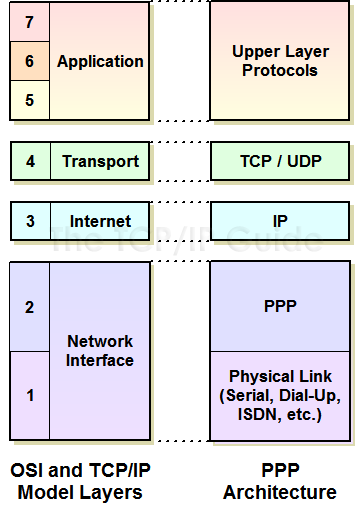
\includegraphics[width=0.3\textwidth]{img/ppplayers}
 \caption{Eingliederung in OSI/TCP-Modell (Entnommen von \cite{ppposi})}
 \label{fig:osi}
\end{figure}

\subsection{Rahmenbildung}
Die Rahmenbildungsmethode von PPP kennzeichnet das Ende und den Anfang des nächsten Rahmens eindeutig und kann Fehler erkennen. Es ist ähnlich dem \textit{High-Level Data Link Control} (HDLC) Protokoll aufgebaut, ist statt diesem aber nicht Bit- sondern Byte-Orientiert. Dies bedeutet, dass immer eine gerade Anzahl von Bytes verwendet wird. Obwohl PPP auch zuverlässige Übertragungen bieten kann wird meist ein Nicht-Nummerierter, also unbestätigter Datentransfer genutzt.

% bisschen klein, evtl größer neu machen
\begin{figure}[h!]
 \centering
  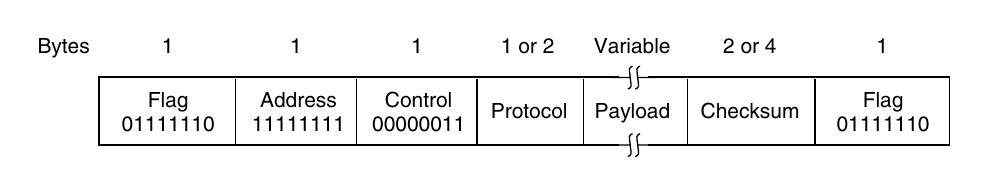
\includegraphics[width=0.5\textwidth]{img/ppprahmen}
 \caption{PPP-Rahmen im Nicht-Nummerierten Modus (Entnommen aus \cite{compnetzw})}
 \label{fig:ppprahmen}
\end{figure}

Im Folgenden wird der detaillierte Aufbau eines PPP--Rahmens erläutert (siehe Abbildung \ref{fig:ppprahmen}).\\
Das 1. Byte stellt dabei das sogenannte \textit{Flagbyte} dar, welches den Anfang und das Ende des Rahmens kennzeichnet und immer aus den Bits \texttt{01111110} (hexadezimal \texttt{0x7E}) besteht. Sollte im Payload die selbe Bitfolge vorkommen, wird diese vor dem Versand ``escaped'', also markiert und umgewandelt (auch Bytestopfen genannt). Hierfür wird diesem Byte ein weiteres Escapebyte vorangestellt (\texttt{0x7D}) und anschließend das Eigentliche mit \texttt{0x20} XOR-verknüpft. Somit wird aus dem Flagbyte im Payload \texttt{0x7D 0x5E}. Mithilfe des Escaping kann einfach nach Anfang und Ende des Rahmens gesucht werden. Beim Auslesen wird nach dem Flagbyte \texttt{0x7D} gesucht, selbiges bei Fund gelöscht und das nachfolgende wieder mit \texttt{0x20} XOR--verknüpft. Zwischen zwei Rahmen wird nur ein Flagbyte benötigt um beide abzugrenzen.\\
Das 2. Byte ist das \textit{Addressbyte}, das immer auf \texttt{11111111} gesetzt ist um an allen Stationen durchgelassen zu werden. Ähnlich einem IP--Broadcast muss somit keine spezifische Adresse zugewiesen werden.\\
Nach dem \textit{Addressbyte} folgt das \textit{Controlbyte}, welches immer mit \texttt{00000011} gesetzt ist, um anzugeben, dass der Rahmen unnummeriert ist. Bei schlechten Verbindungen mit Verlusten, wie z.\,B. drahtlose Netzwerke sollte die Rahmennummerierung aktiviert werden. Da \textit{Addressbyte} und \textit{Controlbyte} meist konstant sind, können Teilnehmer aushandeln die beiden Bytes nicht zu nutzen, letztlich also den Overhead der Rahmen zu vermindern.\\
Das folgende Feld bezeichnet das Protokoll des sich im Payload befindenden Paket. Bitfolgen die mit einer 1 beginnen (ab \texttt{0x8000}), werden für PPP--Verbindungsprotokolle verwendet (z.\,B. LCP, NCP). Bitfolgen beginnend mit einer 0 bezeichnen Protokolle der Vermittlungsschicht (Schicht 3): IPv4/IPv6, aber auch z.\,B. IPX oder Appletalk. Das Feld ist standardmäßig 2 Byte groß, kann aber per LCP auch auf 1 Byte heruntergesetzt werden.\\
Der Payload beinhaltet die eigentlichen Daten, also Pakete anderer Protokolle. Seine Länge beträgt standardmäßig 1500~Byte, kann aber auch per LCP auf eine andere Größe vereinbart werden. Sind die zu übertragenen Daten kleiner als die definierte Payload--Größe, so kann mittels Padding aufgefüllt werden.
%TODO Beispielwerte für Protokolle?
Nach dem Payload folgt eine Checksumme (CRC), die über die Felder Address, Control, Protokoll und den Payload berechnet wird. Das Feld der Checksumme ist standardmäßig 2 Byte groß, kann aber auch auf 4 Byte verhandelt werden (CRC32). Durch diese Checksumme können Übertragungsfehler effektiv entdeckt werden.

\subsection{Unterprotokolle zur Verbindungssteuerung und Aushandeln von Optionen}
\paragraph{Link Control Protocol}
Das \textit{Link Control Protocol} (LCP) dient zum Aufbau, Konfiguration und Prüfung von PPP--Verbindungen. Zur Konfiguration dienen diverse Optionen, die in LCP--Paketen im Payload von PPP--Rahmen übertragen werden. Der initiierende Rechner schlägt Optionen vor, die vom Kommunikationspartner entweder angenommen oder komplett bzw. teilweise abgelehnt werden können. Mögliche Optionen sind u.\,a. die \textit{Maximum Receive Unit} (MRU), das Authentifizierungsprotokoll oder das Qualitätsprotokoll. Ersteres legt die maximale zu übermittelnde Paketgröße fest. Mögliche Authentifizierungsprotokolle sind z.\,B. das \textit{Password Authentication Protocol} (PAP) oder das \textit{Challenge Handshake Authentification Protocol} (CHAP). Über ein optionales Qualitätsprotokoll können Daten zur Verbindungsqualität ausgetauscht werden. Daneben gibt es noch eine Vielzahl weiterer Optionen, die sich z.\,B. um Komprimierung, Nummerierung oder Identifikation kümmern (LCP Erweiterungen).
\paragraph{Network Control Protocol}
Das \textit{Network Control Protocol} (NCP) enthält verschiedene Protokolle zur Aushandlung von Ende--zu--Ende Verbindungsoptionen der Teilnehmer. Am weitesten verbreitet ist dabei das \textit{Internet Protocol Control Protocol} (IPCP) für IPv4. Hierüber können Optionen wie IP--Adresse, Gateway, DNS--Server und Kompression ausgehandelt werden. Damit ist IPCP über Wählverbindungen in seiner Funktion ähnlich dem \textit{Dynamic Host Control Protocol} (DHCP) in Ethernet--Netzwerken.
Neben IPCP gibt es weitere NPCs für andere Protokolle der Vermittlungsschicht beispielsweise IPV6CP für IPv6, IPXCP für IPX oder ATCP für Appletalk.


\section{Kommunikationsabläufe}
Das PPP eignet sich für die Übertragung über eine Vielzahl an Physical Layer Protokollen.
Hierzu zählen unter anderem  Synchronous Optical Network (SONET), GPRS-/UMTS oder auch
in Verbindung mit Ethernet über die weit verbeitete PPPoE-Variante für die Übertragung
über Direct Subscriber Line (DSL) Anschlüsse\cite{IEEEhowto:kopka}.
An dieser Stelle wird exemplarisch der Kommunikationsablauf anhand von PPPoE aufgezeigt.
\subsection{PPP over Ethernet}
Das PPPoE Protokoll ist in RFC 2516 spezifiziert und wurde ursprünglich
von den Firmen UUNET Technologies, Redback Networks und RouterWare entwickelt \cite{RFC2516}.
PPPoE ermöglicht die Übertragung von PPP-Paketen auf Basis von Ethernet, wodurch
die Authentifizierungsfunktionen von PPP mit den
simultanen Zugriffsmöglichkeiten des Ethernet kombiniert werden.
Die Notwendigkeit für PPPoE resultierte aus dem Anfang dieses Jahrtausends
einhergehenden Einzugs der DSL-Technologie und der notwendigen Umstrukturierung
der benötigten Software und Hardware. Ziel war es, ein Protokoll zu entwickeln,
welches die bis dahin vorherrschende Einwahl-Verfahren möglichst kostengünstig
ersetzt. Mit PPPoE war es einerseits möglich die bis dahin bestehenden Software-Stacks für PPP
mit minimalen Anpassungen weiter zu verwenden und ließ sich andererseits mit einfacher
und damit günstiger Hardware umsetzen\cite{dslapp}.
Eines der Haupteinsatzgebiete von PPPoE sind somit Breitbandzugänge über DSL-Anschlüsse,
Wireless-Zugängen oder Kabelmodems und wird
auch von vielen Internet Service Providern (ISP) zu diesem Zweck eingesetzt \cite[p.88]{cisconut}.\\
%
Der strukturelle Aufbau eines typischen PPPoE-Pakets ist in Abbildung \ref{fig:PPPoE_Bild} zu sehen.
\begin{figure}[h!]
 \centering
  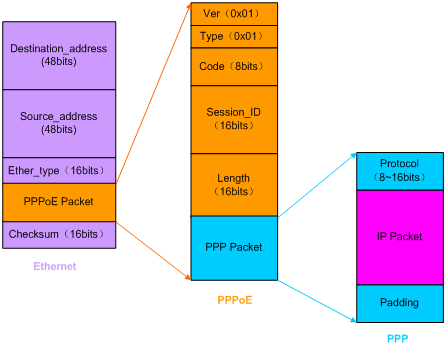
\includegraphics[width=0.5\textwidth]{img/pppoe_aufbau.jpg}
 \caption{Aufbau eines PPPoE-Pakets (Entnommen von \cite{PPPoEBild})}
 \label{fig:PPPoE_Bild}
\end{figure}
Hierbei ist die Verschachtelung der Protokolle der einzelnen Layer zu erkennen: Die unterste
Ebene bildet Ethernet, gefolgt von PPPoE zur PPP bis zum Internet Protokoll.
Der Aufbau von Ethernet und IP-Paketen wird als bekannt vorausgesetzt und hier nicht näher erläutert.\\
%
Die Bedeutung der PPPoE header ist in Tabelle \ref{tab:PPPoE_fields} dargestellt.
%
\begin{figure}[h!]
\begin{tabular}{|l|p{6.5cm}|}
\hline 
Ver & Verwendete Version des PPPoE, immer 1\\ 
\hline 
Type & Verwendeter Typ des PPPoE, immer 1\\ 
\hline 
Code & Typ des PPPoE\-Pakets: 0x00 = Sitzungsdaten; 0x09 = PADI; 0x07 = PADO oder PADT;
0x19 = PADR; 0x65 indicates PADS\\ 
\hline 
Session\_ID & Eindeutiger identifier einer PPP\-Sitzung\\ 
\hline 
Length & Länge des PPPoE\-Payloads\\ 
\hline 
Protocol & Protokolltyp des nächsten Layers\\ 
\hline
\end{tabular}
\end{figure}
% TODO: scheiß label für Tabelle???
\label{tab:PPPoE_fields}
%
Der Ablauf einer PPPoE-Verbindung teilt sich in die drei Phasen Discovery, Session und Terminate
ein. Diese werden in Abbildung \ref{fig:PPPoEsequenz1} in den folgenden Abschnitten näher erläutert (vgl. \cite{RFC2516}).\\
%
\begin{figure}[h!]
 \centering
  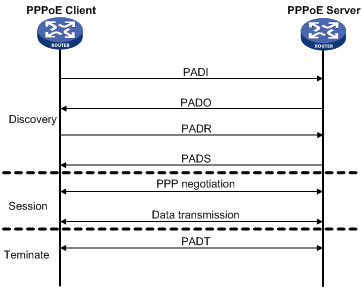
\includegraphics[width=0.5\textwidth]{img/pppoe_sequenz1.png}
 \caption{Ablauf einer PPPoE-Session (Entnommen aus \cite{PPPoEBild})}
 \label{fig:PPPoEsequenz1}
\end{figure}
\subsubsection{Discovery}
Das Ziel dieser Phase ist das Auffinden der MAC-Adresse des Servers (auch Concentrator genannt)
sowie das Ableiten einer PPPoE Session-ID durch den Client (auch Host genannt).
Abhängig von der Topologie können sich mehrere Server im Netzwerk befinden, welche in
dieser Phase durch den Client entdeckt werden. Die Discovery-Phase selbst ist zustandslos, d.h.
auf Seiten aller Kommunikationen werden keine Verbindungsinformationen gespeichert.\\
Das erste gesendete PPPoE Active Discovery Initiation (PADI) Paket stellt ein Broadcast
an alle im Netzwerk vorhanden Server dar. Dieses enthält den Namen des vom Client
angefragten Service, auf welches Server mit einem
PPPoE Active Discovery Offer (PADO) Paket antworten. Das Antwortpaket
hat als Zieladresse die des Clients und enthält neben dem Namen des Servers optional
weitere vom Server angebotene Service-Namen. Es folgt ein PPPoE Active Discovery Request (PADR) Paket
mit welchem der Client den von ihm nun gewählten Server und Service unter allen
gefundenen direkt adressiert. Nach Erhalt des PADR beginnt der Server mit dem Aufbau
einer PPP Session und bestätigt dies mit einem PPPoE Active Discovery Session-confirmation (PADS) Paket.
Diese enthält auch eine Session-ID, welche die folgende Session eindeutig Identifiziert.
\subsubsection{Session}
In der Sitzungsphase erfolgt die weitere Konfiguration der Verbindung, die Authentifikation des
Clients sowie der eigentliche Datenaustausch. Dieser ist im Gegensatz zur Discovery und Terminate
Phase PPP-spezifisch und in Abbildung \ref{fig:PPPoEsequenz2} genauer dargestellt.
%
\begin{figure}[h!]
 \centering
  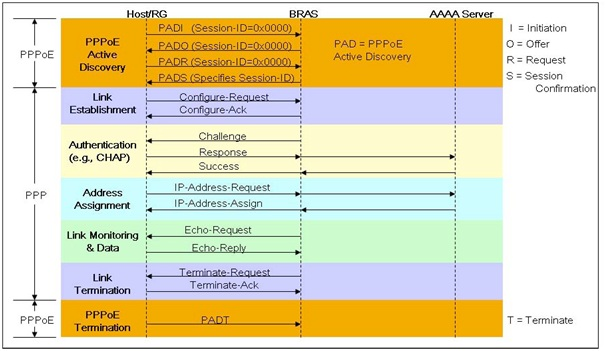
\includegraphics[width=0.5\textwidth]{img/pppoe_sequenz2.jpg}
 \caption{PPP-Spezifischer Teil eines PPPoE-Verbindungsaufbaus (Entnommen aus \cite{pppoesequenz2})}
 \label{fig:PPPoEsequenz2}
\end{figure}
%
TODO: Ablauf für PPP-Session beschreiben.\\
Hierbei wird zunächst ein Link Establishment über das Link Control Protocol (LCP) durchgeführt.
Daraufhin erfolgt eine optionale Authentifikation entweder über das Password Authentication Protocol (PAP)
oder dem Challenge-Handshake Authentication Protocol (CHAP). Bei einem DSL-Anschluss entspricht dies
dem Nachweis der Kenntnis der vom ISP mitgeteilten Anschlussdaten. Es erfolgt die Zuweisung einer
Netzwerk-Adresse über das Network Control Protocol (NCP) und im Anschluss der Austausch der
eigentlichen Nutzdaten. Die Verbindung kann nun jederzeit terminiert werden, z.B.
aufgrund von Inaktivität oder einem Session-Timeout.
%
%
\begin{figure}[h!]
 \centering
  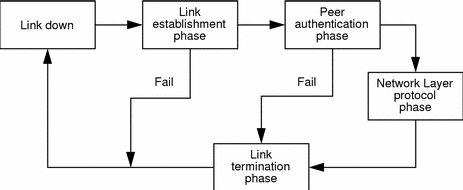
\includegraphics[width=0.5\textwidth]{img/ppp_linkstates.png}
 \caption{Phasen der PPP-Session (Entnommen aus \cite{pppoesequenz2})}
 \label{fig:PPPoEsequenz2}
\end{figure}
%
%
\subsubsection{Terminate}
Die PPPoE Verbindung kann jederzeit von beiden Kommunikationspartner beendet werden. Hierfür sendet
der Client oder der Server ein PPPoE Active Discovery Terminate (PADT) Paket. Nach Erhalt dieses
Pakets ist kein weiterer Datenaustausch über die Session erlaubt.
%


\section{Fazit} 
Wie in der Einf\"uhrung erw\"ahnt, war das Point-to-Point Protocol notwendig, da die damals aktuellen Standards nicht alle mittlerweile ben\"otigten Anforderungen erf\"ullen konnten. Durch die einfache Handhabung der aufgebauten verbindung f\"ur Netzwerk-Schicht-Protokolle, ist vermutlich auch die grosse Verbreitung des Protokolls zu erkl\"aren. Bei fast allen M\"oglichkeiten eine Internetverbindung aufzubauen (sei es \"uber DSL oder im Mobilfunknetz) wird PPP als Einw\"ahlprotokoll genutzt. Zwar wird im Kabelnetz mittlerweile ein anderes Protokoll verwendet, doch durch die einfache Umsetzung des Point-to-Point Protokolls wird es wahrscheinlich noch einige Jahre der Standard beim Verbinden mit dem ISP sein.

\appendices 
\section*{Acknowledgment} 
The authors would like to thank...deiner Mudda
% Can use something like this to put references on a page 
% by themselves when using endfloat and the captionsoff option. 
\ifCLASSOPTIONcaptionsoff 
  \newpage 
\fi
\begin{thebibliography}{1} 
\bibitem{IEEEhowto:kopka} 
H.~Kopka and P.~W. Daly, \emph{A Guide to \LaTeX}, 3rd~ed.\hskip 1em plus 
  0.5em minus 0.4em\relax Harlow, England: Addison-Wesley, 1999. 
Andrew S. Tanenbaum: Computer Networks, 5.th edition, Prentice Hall, 2011
James F. Kurose / Keith W. Ross, Computernetzwerke, Pearson, 2012

%RFC 1661 – Point-to-Point Protocol (PPP) July 1994;
%RFC 1662 – Point-to-Point Protocol in HDLC-like Framing
%RFC 1962, PPP Compression Control Protocol (CCP)
%RFC 1963, PPP Serial Data transport Protocol
%RFC 1990, The PPP Multilink Protocol (MP)
%RFC 1994, PPP Challenge Handshake Authentication Protocol (CHAP)
%RFC 2153, Informational, PPP Vendor Extensions
%RFC 2284, PPP Extensible Authentication Protocol (EAP)
%RFC 2364, PPP over ATM
%RFC 2516, PPP over Ethernet
%RFC 2615, PPP over SONET/SDH
%RFC 2686, The Multi-Class Extension to Multi-Link PPP
%RFC 2687, Proposed Standard, PPP in a Real-time Oriented HDLC-like Framing
%RFC 5072, IP Version 6 over PPP
%RFC 5172, Negotiation for IPv6 Datagram Compression Using IPv6 Control Protocol
%RFC 6361, PPP Transparent Interconnection of Lots of Links (TRILL) Protocol Control Protocol
\bibitem{RFC2516} A Method for Transmitting PPP Over Ethernet (PPPoE) (IETF RFC2516), \newblock L. Mamakos, \newblock K. Lidl, \newblock J. Evarts, \newblock 1999.
\bibitem{RFC2637} Point-to-Point Tunneling Protocol (IETF RFC 2637), \newblock K. Hamzeh, \newblock The Internet Society, \newblock Juli, \newblock 1999.
\bibitem{RFC1661} Point-to-Point Protocol (IETF RFC 1661), \newblock W. Simpson, \newblock The Internet Society, \newblock Juli, \newblock 1994.
\bibitem{RFC2364} Point-to-Point Protocol over AAL5 (IETF RFC 2364), \newblock  G. Gross, \newblock The Internet Society, \newblock Juli, \newblock 1998.
\bibitem{RFC2516} Point-to-Point Protocol over Ethernet (IETF RFC 2516), \newblock  L. Mamakos, \newblock The Internet Society, \newblock Februar, \newblock 1999.
\bibitem{RFC3256} The DOCSIS (Data-Over-Cable Service Interface Specifications) Device Class DHCP (Dynamic Host Configuration Protocol) Relay Agent Information Sub-option (IETF RFC 3256), \newblock  D. Jones
, \newblock The Internet Society, \newblock April, \newblock 2002.
\bibitem{PPP-Bild} Veranschaulichung einer PPP-Verbindung, \newblock Vicomsoft, \newblock http://www.vicomsoft.com/learning-center/pppoe/
\bibitem{cisconut} Cisco IOS in a Nutshell \newblock James Boney, \newblock O'Reilly Media \newblock 2005
\bibitem{dslapp} Implementation and Applications of DSL Technology, \newblock Philip Golden Hervé Dedieu, \newblock Krista S. Jacobsen, \newblock 1998
%\bibitem{RFC1055} http://tools.ietf.org/html/rfc1055
\bibitem{PPPoEBild} Aufbau eines PPPoE-Pakets,\newblock H3C \newblock http://www.h3c.com/portal/Products\_\_\_Solutions/Technology/WAN/Technology\_White\_Paper/200911/654415\_57\_0.htm
\bibitem{pppoesequenz1} Ablauf eine PPPoE-Verbindung,\newblock xxx \newblock http://
\bibitem{pppoesequenz2} PPP-Spezifischer Teil eines PPPoE-Verbindungsaufbaus,\newblock xxx \newblock http://
\bibitem{ppposi} Eingliederung von PPP im OSI--Modell,\newblock Abrufdatum: 29.05.2014, \newblock http://www.tcpipguide.com/free/
\bibitem{compnetzw} Computernetzwerke, \newblock Andrew S. Tanenbaum,  \newblock Pearson Verlag, \newblock 5. Auflage, \newblock 2012.
\end{thebibliography} 
\end{document} 
